L'application se lance sur un double-clic sur l'exécutable.

\section{Se connecter}
\subsection{IHM de connexion}
La première fen\^etre permet de se connecter au SGBD (figure \ref{se_connecter_gui}).
\begin{figure}[!h]
\centering
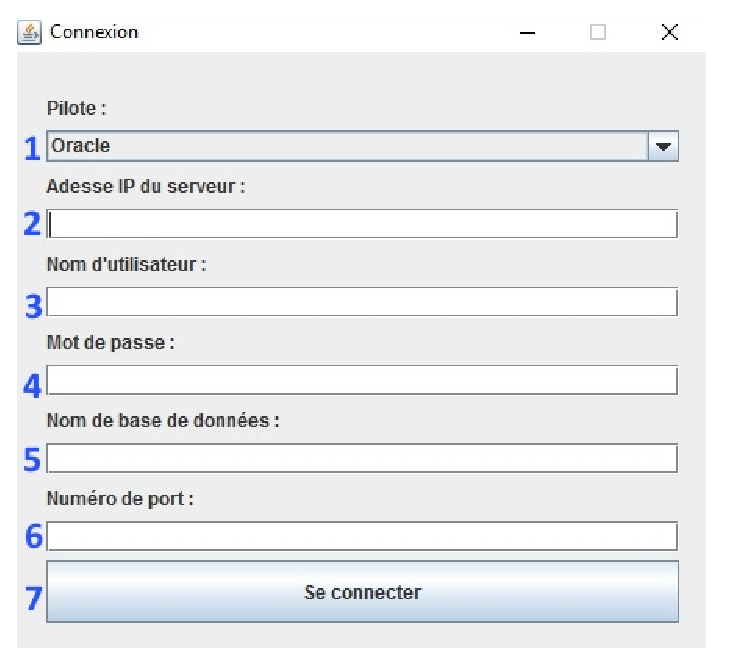
\includegraphics[width=10cm]{./images/manuel/se_connecter.eps}
\caption{\gls{ihm}* - Se connecter}
\label{se_connecter_gui}
\end{figure}

Pour se connecter, renseigner les différents champs présents dans la fen\^etre.

\begin{enumerate}
\item choix du \gls{sgbd}* (Oracle, MySQL).
\item Adresse IP du serveur où est stockée votre base de données.
\item Nom d'utilisateur utilisé pour vous connecter à votre base de données. 
\item Mot de passe utilisé pour vous connecter à votre base de données.
\item Nom de la base de données.
\item Numéros de port du serveur ou est stockée votre base de données.
\item Cliquer sur le bouton \textbf{se connecter} pour vous connecter au serveur.
\end{enumerate}

\subsection{Connexion aux serveurs de l'IUT}
Si vous êtes un étudiant de l'IUT de Montpellier.

\subsubsection{Oracle}
\begin{itemize}
\item SGBD : Oracle
\item Adresse IP : 162.38.222.149
\item Nom d'utilisateur : <nom-de-famille><première-lettre-du-prenom>
\item Mot de passe : <votre-INE>
\item Nom de la base de données : IUT
\item Numéros de port : 1521 \\
\end{itemize}

\subsubsection{MySQL}
\begin{itemize}
\item SGBD : MySQL
\item Adresse IP : 162.38.222.142
\item Nom d'utilisateur : <nom-de-famille><première-lettre-du-prenom>
\item Mot de passe : <votre-INE>
\item Nom de la base de données : <nom-de-famille><première-lettre-du-prenom>
\item Numéros de port : 3306
\end{itemize}

\section{Créer une table}
Dans le menu principal de l'application, cliquer sur le bouton \textbf{\gls{ldd} : créer tables} pour ouvrir la fen\^etre de création de tables (figure \ref{creer_table_gui}).

\begin{figure}[!h]
\centering
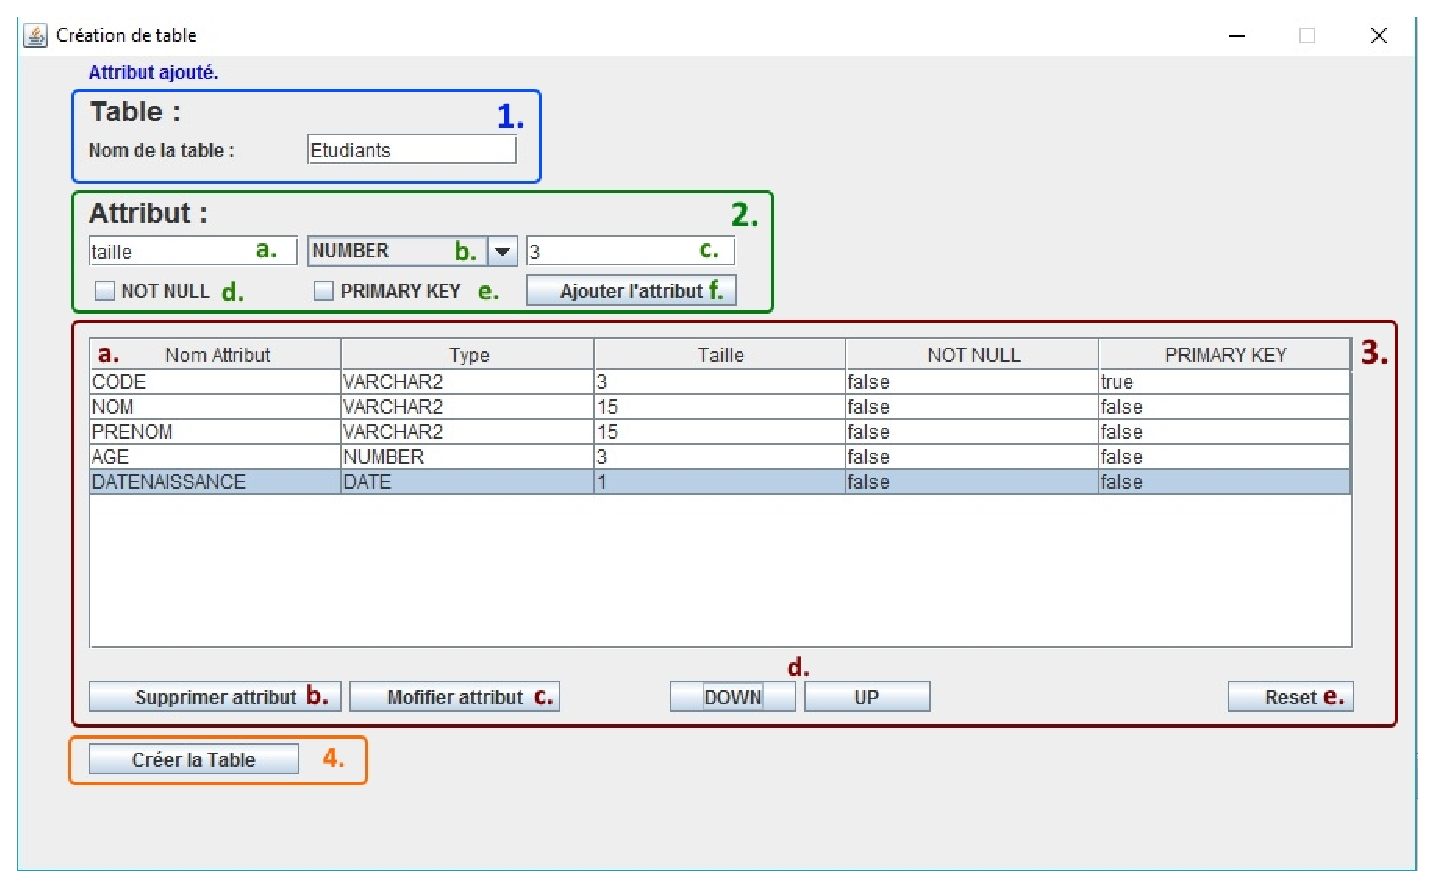
\includegraphics[width=14cm]{./images/manuel/creer_table.eps}
\caption{IHM - Créer table}
\label{creer_table_gui}
\end{figure}

\begin{enumerate}
\item Nom de ta table - \textit{ex : Etudiants}

\item Gestion des caractéristiques d'un attribut :
\begin{enumerate}
\item Nom - \textit{ex : codeEtudiant}
\item Type - \textit{ex : VARCHAR2}
\item Taille - \textit{ex : 15}
\item A cocher pour que l'attribut ne soit jamais null.
\item A cocher pour que l'attribut soit membre de la clée primaire de votre table.
\item Cliquer sur le bouton \textbf{Ajouter l'attribut} pour tenter d'ajouter un attribut à la table.
\end{enumerate}

\item Gestion des attributs ajoutés :
\begin{enumerate}
\item Tableau contenant les attributs ajoutés avec le bouton \textbf{Ajouter l'attribut}.
\item Cliquer sur le bouton \textbf{Supprimer l'attribut} pour supprimer l'attribut sélectionné dans le tableau.
\item Cliquer sur le bouton \textbf{Modifier l'attribut} pour modifier l'attribut sélectionné dans le tableau. 
Les caractéristiques de l'attribut sélectionné sont à modifier dans la zone de gestion des caractéristiques d'un attribut. 
Vous pouvez ensuite valider ou annuler votre modification.
\item Cliquer sur les boutons \textbf{UP/DOWN} pour modifier l'ordre des attributs dans le tableau. 
\item Cliquer sur le bouton \textbf{Reset} pour remettre à zéro la fen\^etre de création.
\end{enumerate}

\item Cliquer sur le bouton \textbf{Créer la table} pour créer la table.
\end{enumerate}


\section{Modifier une table}
Dans le menu principal de l'application, cliquer sur le bouton \textbf{LDD : modifier tables} pour ouvrir la fenêtre de modification de tables (figure \ref{modifier_table_gui}).


\begin{figure}[!h]
\centering
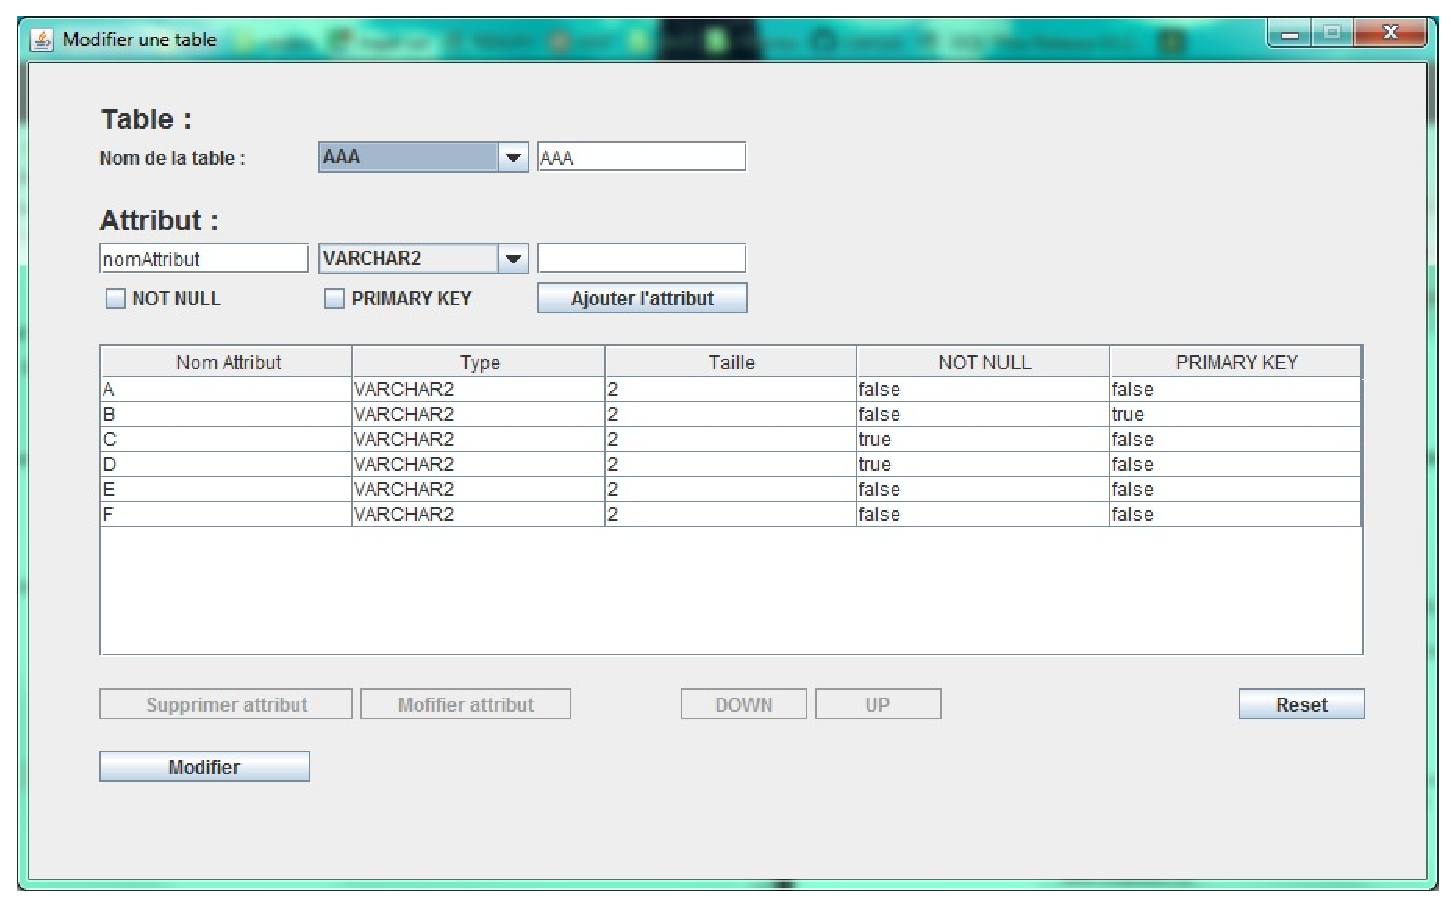
\includegraphics[width=10cm]{./images/manuel/modifier_tables.eps}
\caption{IHM - Modifier une table}
\label{modifier_table_gui}
\end{figure}

Cette fenêtre est identique à la fenêtre de création d'une table, à la différence qu'il est possible de sélectionner une table déjà existante dans la \bdd. 

Il est possible de modifier une table existante avec le bouton \textbf{modifier}, sans perdre de données mais il est possible que certaines soient perdues lors de la modification, notamment dans les cas suivants :
\begin{itemize}
\item suppression d'un attribut clée étrangère couplé avec un second attribut
\item modification du type de l'attribut pouvant altérer les données.
\end{itemize}





\section{Supprimer une table}
Dans le menu principal de l'application, cliquer sur le bouton \textbf{LDD : supprimer tables} ouvre la fen\^etre de suppression de tables (figure \ref{supprimer_table_gui}).

\begin{figure}[!h]
\centering
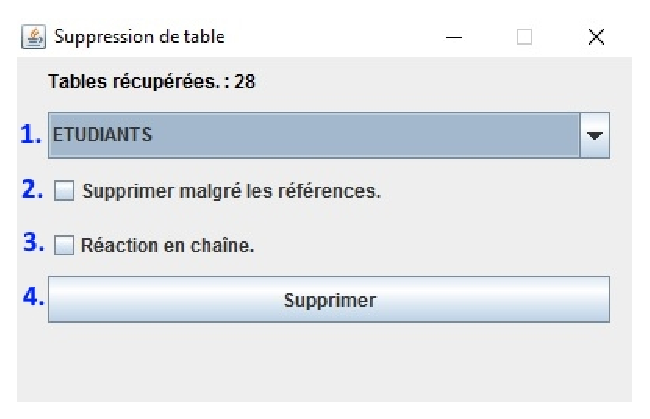
\includegraphics[width=8cm]{./images/manuel/supprimer_table.eps}
\caption{IHM - Supprimer une table}
\label{supprimer_table_gui}
\end{figure}

\begin{enumerate}
\item Choisir la table à supprimer.
\item A cocher pour supprimer sans prendre en compte les références des autres tables sur celle à supprimer.
\item A cocher pour supprimer la table sélectionnée puis toutes celles qui font référence à cette table et ceci récursivement.
\item Cliquer sur le bouton \textbf{Supprimer} pour tenter la suppression de la table.
\end{enumerate}

\section{Requ\^etes SQL}
Dans le menu principal de l'application, cliquer sur le bouton \textbf{\gls{sql}}* pour ouvrir la fen\^etre du mode requ\^etes SQL (figure \ref{sql_gui}).
\begin{figure}[!h]
\centering
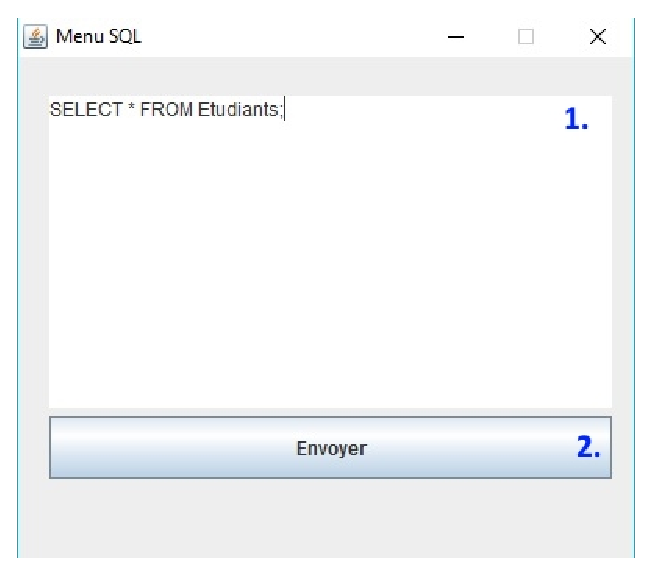
\includegraphics[width=6cm]{./images/manuel/sql.eps}
\caption{IHM - SQL}
\label{sql_gui}
\end{figure}

\begin{enumerate}
\item Ecrire la requ\^ete dans la zone de saisie - \textit{ex : SELECT * FROM Etudiants;} 
\item Cliquer sur le bouton \textbf{Envoyer} pour tenter d'exécuter la requ\^ete.
Une fenêtre (figure \ref{sql_result_gui}) s'ouvre indiquant le résultat de la requ\^ete si la syntaxe est correcte.
\end{enumerate}

\begin{figure}[!h]
\centering
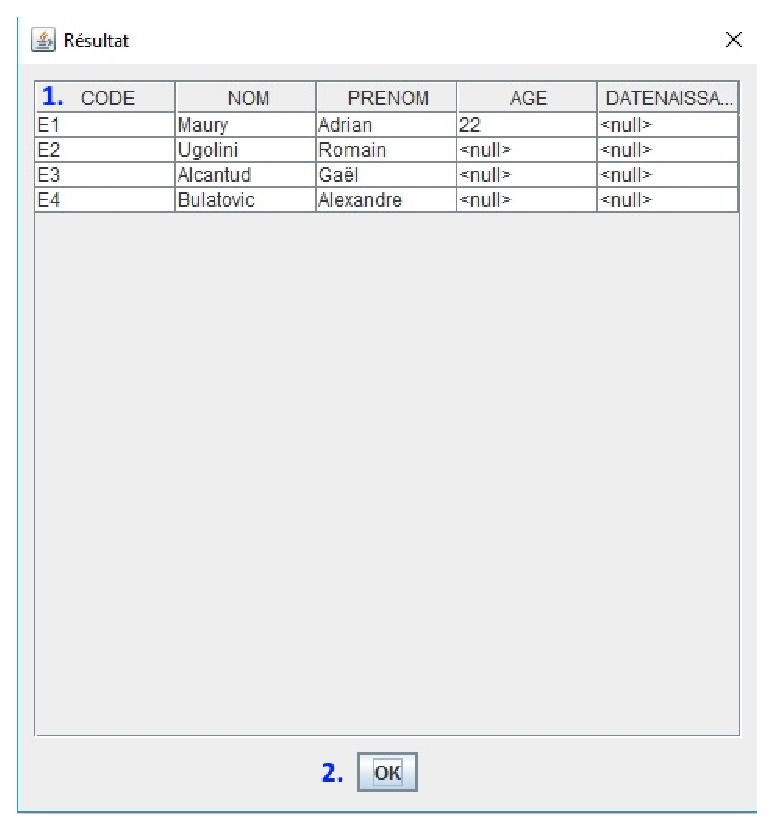
\includegraphics[width=8cm]{./images/manuel/sql_result.eps}
\caption{IHM - Résultat SQL}
\label{sql_result_gui}
\end{figure}

\begin{enumerate}
\item Résultat de la requ\^ete.
\item Cliquer sur le bouton \textbf{OK} pour fermer la fenêtre de résultat.
\end{enumerate}

\section{CRUD les tuples des tables}
Dans le menu principal de l'application, cliquer sur le bouton \textbf{\gls{crud}}* pour ouvrir la fen\^etre de gestion des \glspl{tuple}* des tables (figure \ref{crud_gui}).
\begin{figure}[!h]
\centering
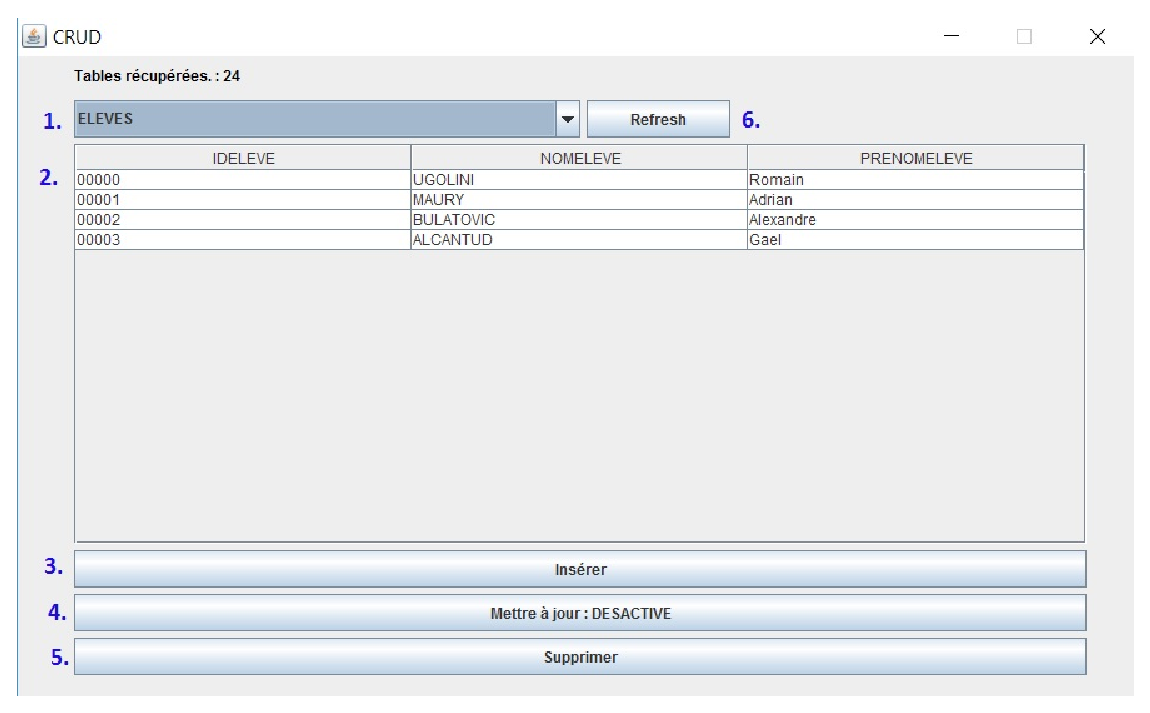
\includegraphics[width=12cm]{./images/manuel/crud.eps}
\caption{IHM - CRUD}
\label{crud_gui}
\end{figure}

\begin{enumerate}
\item Choisir la table.
\item Tableau contenant les différents tuples de la table sélectionnée.
\item Cliquer sur le bouton \textbf{Insérer} pour ajouter un tuple à la table. Il faut ensuite remplir les informations du nouveau tuple
dans la ligne vide qui s'est ajouté au tableau.
\item Cliquer sur le bouton \textbf{Mettre à jour} pour modifier un tuple de la table. Il faut ensuite modifer les informations du tableau et 
appuyer sur la touche entrée à chaque modification. Quitter le mode modification en cliquant une nouvelle fois sur le bouton \textbf{Mettre à jour}.
\item Cliquer sur le bouton \textbf{Supprimer} pour supprimer le tuple selectionné.
\item Cliquer sur le bouton \textbf{Refresh} pour rafraichir la vue et que la supression soit prise en compte.
\end{enumerate}

\section{Ajouter et Supprimer des contraintes}

Dans le menu principal de l'application, cliquer sur le bouton \textbf{LDD : créer supprimer des contraintes} pour ouvrir la fen\^etre de création et supression de contraintes unique et clées étrangères(figure \ref{contraintes_unique_gui}).

\begin{figure}[!h]
\centering
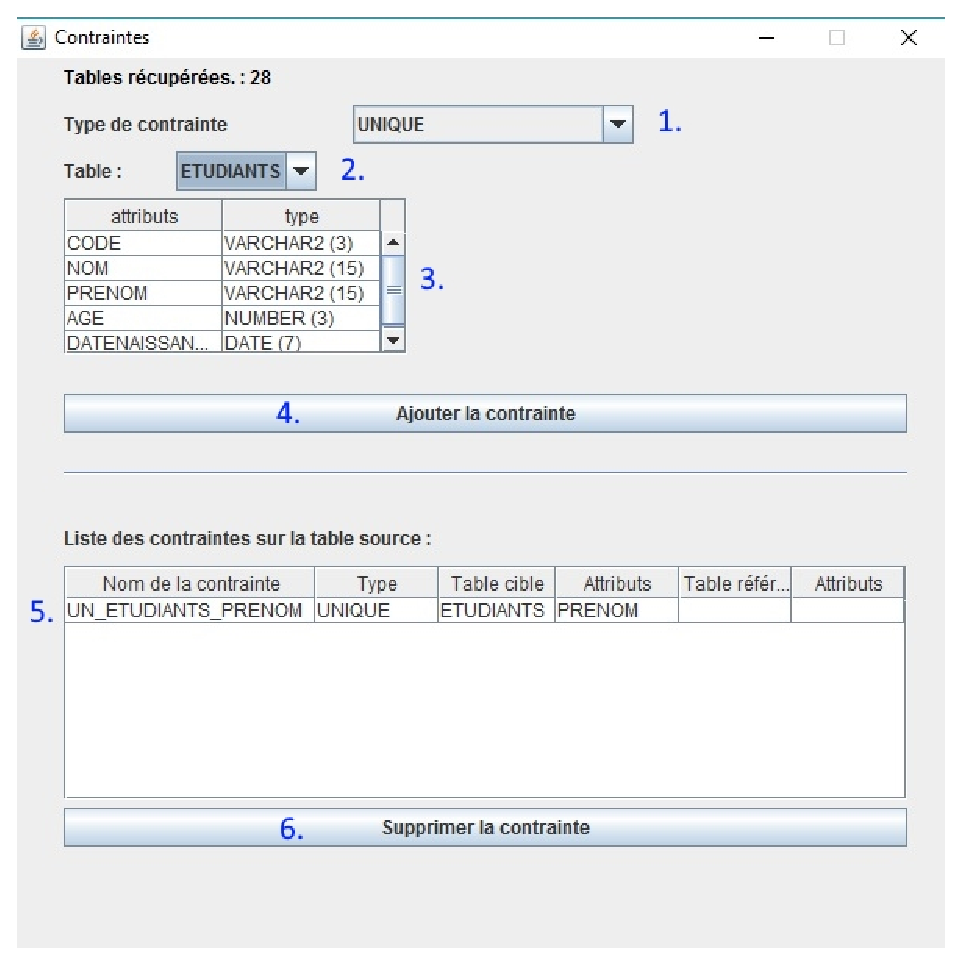
\includegraphics[width=12cm]{./images/manuel/contraintes_unique.eps}
\caption{IHM - Contraintes unique}
\label{contraintes_unique_gui}
\end{figure}

Pour créer une contrainte \textbf{unique} :
\begin{enumerate}
\item Choisir le type de contrainte à ajouter à votre table.
\item Choisir la table.
\item Tableau contenant les attributs de la table. Pour ajouter la contrainte il faut sélectionner des attributs dans ce tableau. La selection multiple de fait à l'aide la la touche CTRL.
\item Cliquer sur le bouton \textbf{Ajouter la contrainte} pour ajouter la contrainte à la table.
\item Tableau contenant les contraintes de la table source.
\item Cliquer sur le bouton \textbf{Supprimer la contrainte} pour supprimer la contrainte de la table et du tableau.
\end{enumerate}

Pour créer une contrainte \textbf{clée étrangère} ( FOREIGN KEY ) :\\
Même déroulement que pour une contrainte unique sauf pour les points 2 et 3 (figure\ref{contraintes_fk_gui}).

\begin{enumerate}
\item Choisir les tables source et destination pour la clée etrangère.
\item Tableaux contenant les attributs de la table source et de la table destination. Pour ajouter la contrainte il faut sélectionner des attributs dans ces tableaux. La selection multiple de fait à l'aide la la touche CTRL. Le nombre d'attributs sélectionnés dans la table source doit être le même que dans la table destination.
\end{enumerate}

\begin{figure}[!h]
\centering
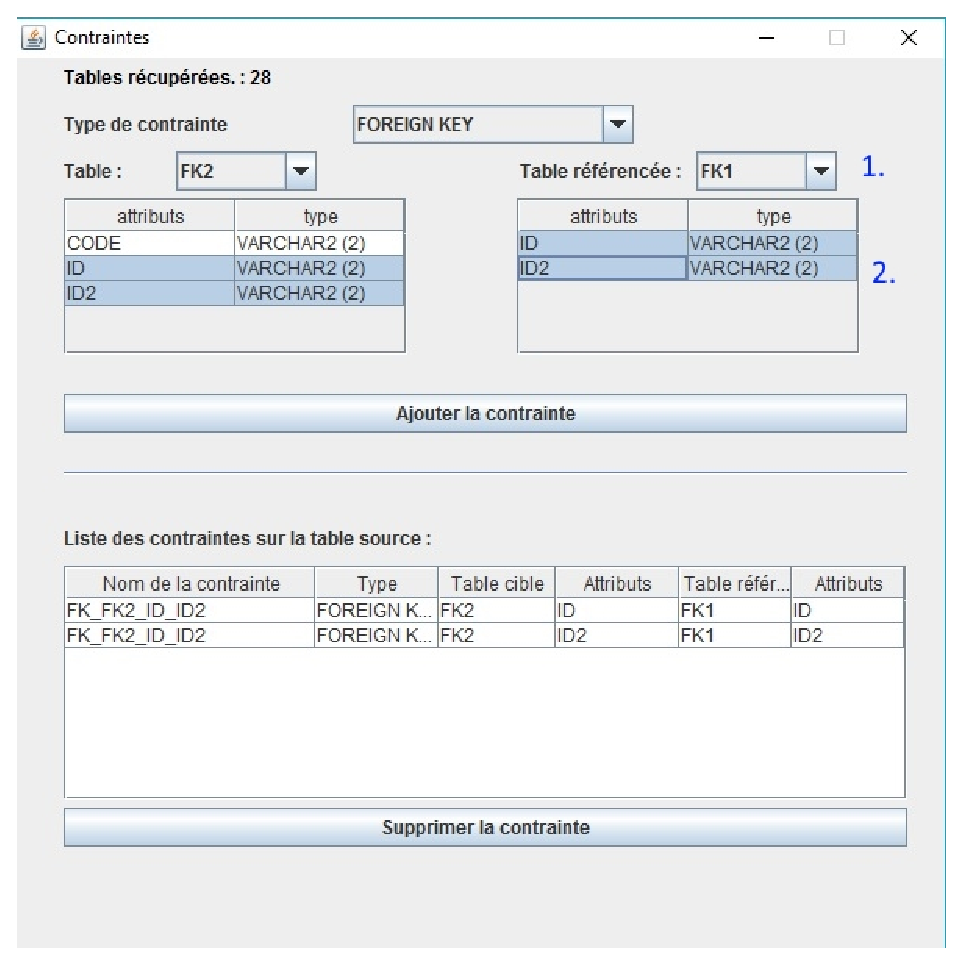
\includegraphics[width=12cm]{./images/manuel/contraintes_fk.eps}
\caption{IHM - Contraintes foreign key}
\label{contraintes_fk_gui}
\end{figure}


\section{Faire des requêtes graphiques : QBE*}

Dans le menu principal de l'application, cliquer sur le bouton \textbf{QBE : Requêtes} pour ouvrir la fenêtre de requêtes graphique(figure \ref{qbe_gui}).

\begin{figure}[!h]
\centering
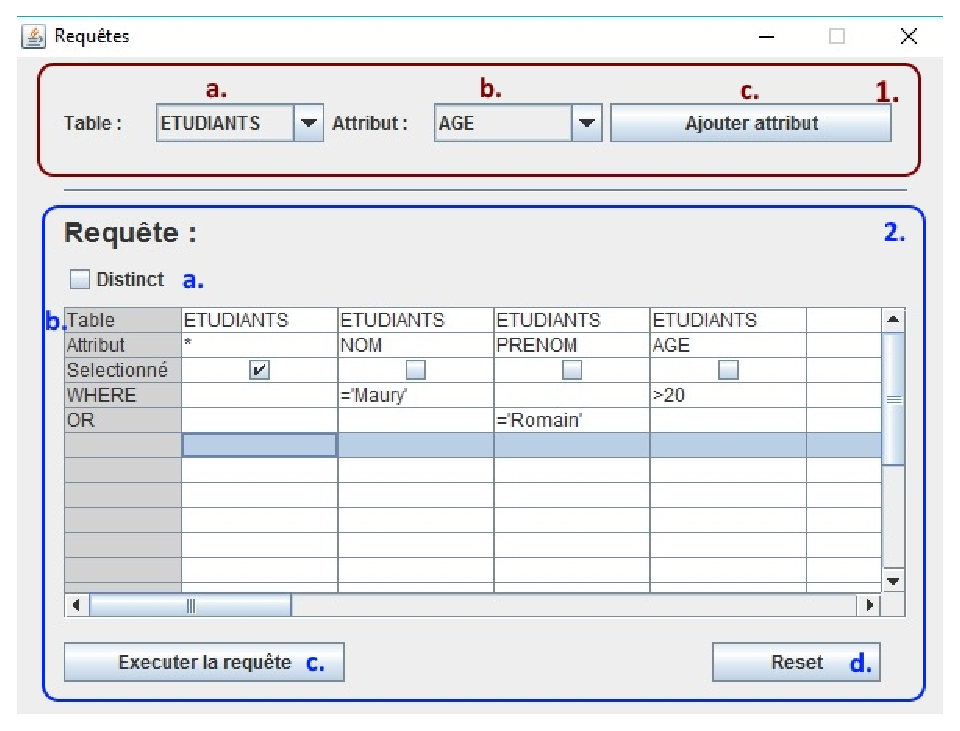
\includegraphics[width=12cm]{./images/manuel/qbe.eps}
\caption{IHM - Requêtes graphique (QBE)}
\label{qbe_gui}
\end{figure}

\begin{enumerate}
\item Ajouter un attribut à la requête :
\begin{enumerate}
\item Choisir la table.
\item Choisir l'attribut ou * pour selectionner tout les attributs.
\item Cliquer sur le bouton \textbf{Ajouter l'attribut} pour ajouter l'attribut à la requête.
\end{enumerate}
\item Modifier les caractéristiques de la requête :
\begin{enumerate}
\item A cocher pour qu'il n'y ai pas de doublon dans le résultat de la requête.
\item Tableau contenant les attributs utilisés dans la requête ainsi que les conditions de sélection pour la requête :
\begin{itemize}
\item Table : nom de la table cible.
\item Attribut : nom de l'attribut cible. ( * pour sélectionner toute la table ).
\item Sélectionné : à cocher pour que l'attribut soit visible dans le résultat de la requête.
\item WHERE : condition de séléction sur un attribut. 
Plusieur conditions sur une même ligne correspondent à l'opérateur logique AND. \\
\textit{Ex (figure \ref{qbe_gui}) : nom = 'Maury' \textbf{AND} age>20}.\\
Plusieur conditions sur des lignes différentes correspondent à l'opérateur logique OR.\\
 \textit{Ex : (nom = 'Maury' AND age>20) \textbf{OR} prenom = 'Romain'}.\\
\end{itemize}
\item Cliquer sur le bouton \textbf{Executer la requête} pour executer la requête.
\item Cliquer sur le bouton \textbf{Reset} pour remettre à zéro la fenêtre.
\end{enumerate}
\end{enumerate}

La fenêtre de résultat de la requête s'ouvre. Cliquer sur le bouton \textbf{OK} pour fermer la fenêtre (figure \ref{qbe_result_gui}).

\begin{figure}[!h]
\centering
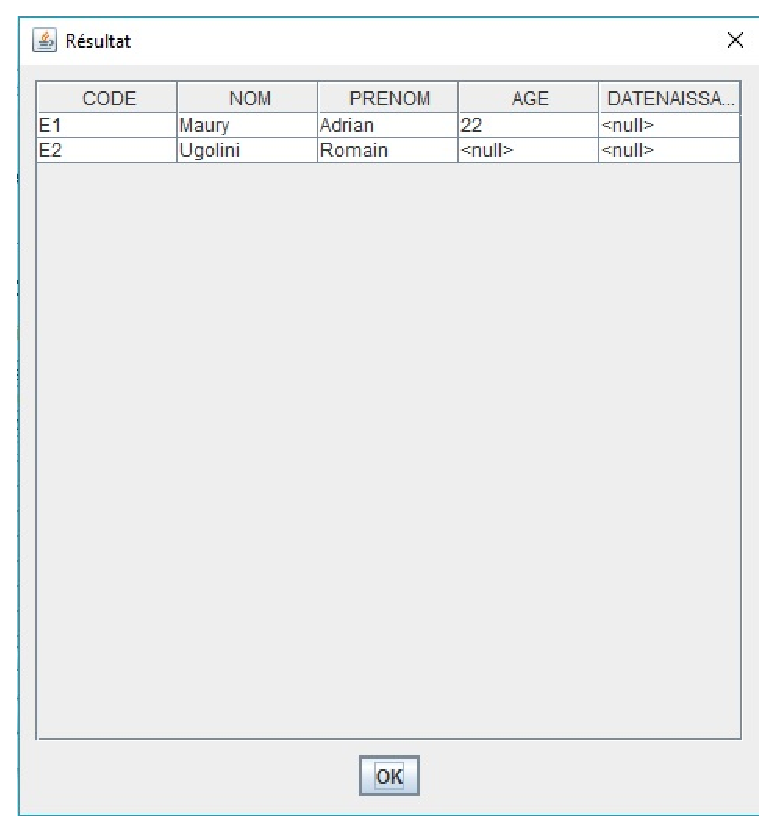
\includegraphics[width=12cm]{./images/manuel/qbe_result.eps}
\caption{IHM - Requêtes graphique (QBE) - Resultat}
\label{qbe_result_gui}
\end{figure}